\documentclass[12pt]{article}%
\usepackage{amsfonts}
\usepackage{fancyhdr}
\usepackage{comment}
\usepackage{mathtools}
\usepackage[a4paper, top=2.5cm, bottom=2.5cm, left=3cm, right=3cm]%
{geometry}
\usepackage{times}
\usepackage{amsmath}
\usepackage{changepage}
\usepackage{amssymb}
\usepackage{listings}
\usepackage{graphicx}%
\setcounter{MaxMatrixCols}{30}
\newtheorem{theorem}{Theorem}
\newtheorem{acknowledgement}[theorem]{Acknowledgement}
\newtheorem{algorithm}[theorem]{Algorithm}
\newtheorem{axiom}{Axiom}
\newtheorem{case}[theorem]{Case}
\newtheorem{claim}[theorem]{Claim}
\newtheorem{conclusion}[theorem]{Conclusion}
\newtheorem{condition}[theorem]{Condition}
\newtheorem{conjecture}[theorem]{Conjecture}
\newtheorem{corollary}[theorem]{Corollary}
\newtheorem{criterion}[theorem]{Criterion}
\newtheorem{definition}[theorem]{Definition}
\newtheorem{example}[theorem]{Example}
\newtheorem{exercise}[theorem]{Exercise}
\newtheorem{lemma}[theorem]{Lemma}
\newtheorem{notation}[theorem]{Notation}
\newtheorem{problem}[theorem]{Problem}
\newtheorem{proposition}[theorem]{Proposition}
\newtheorem{remark}[theorem]{Remark}
\newtheorem{solution}[theorem]{Solution}
\newtheorem{summary}[theorem]{Summary}
\newenvironment{proof}[1][Proof]{\textbf{#1.} }{\ \rule{0.5em}{0.5em}}

\newcommand{\Q}{\mathbb{Q}}
\newcommand{\R}{\mathbb{R}}
\newcommand{\C}{\mathbb{C}}
\newcommand{\Z}{\mathbb{Z}}
\newcommand{\Lagr}{\mathcal{L}}
\newcommand{\Dual}{\mathcal{D}}

\begin{document}
	
	\title{Fall 2021: MAS4112 Final Project\\Support Vector Machine}
	\author{Branislav Kesic}
	\date{\today}
	\maketitle
	
	\section{Introduction}
	A common problem that can be solved in machine learning is the case of classification.  Within classification scenarios, our motivation is to classify data points into two or more categories.  This paper utilizes the method of Support Vector Machines in order to solve a binary classification problem, and further extends the binary classfication case to support 3 or more categories.  The algorithm used was built from scratch using python, where the only libraries used were numpy and pandas.  Furthermore, we will use a soft-margin support vector machine which allows for the classification on non-linearly separable datasets and allows errors in classification, as opposed to a hard-margin support vector machine which fails the task of non-linearly separable datasets.
	
	\section{Support Vector Machines}
	
	\subsection{Binary Classification Intuition}
	The idea behind the Support Vector Machine algorithm is to draw a boundary between 2 different classes in a dataset.  The Support Vector Machine achieves this using the intuition of a hyperplane, which in it's most simple state solves only the binary classification problem between two classes.  We can visualize the hyperplane as a point in 1D, a line in 2D, a plane in 3D, and so on.  The idea of a hyperplane is that we classify a datapoint with "+1" or "-1" corresponding to either of two classes, depending on whether the datapoint falls below or above the hyperplane.  
	
	\subsection{Hinge Loss Cost Function}
	The method for optimizing the support vector machine in this paper builds off of the cost function of hinge loss, and is optimized using sub-gradient descent.  The support vector machine utilizes what is called a margin, where the idea is to maximize the distance between the margin and any data point, in order to maximize the effectiveness of the hyperplane.  The margin extends to both the positive and negative positions of the hyperplane.\\
	
	Consider the follow optimization problem of hinge loss:\\
	
	$\ell(y)=\underset{w,b}{min}$ $\frac{1}{2}||w||^2 + C\sum_{n=1}^{N}\max\{0,1-y_n(<w,x_n>+b)\}$\\\\
	\indent Where w,b represent our weights to be optimized with w being a normal vector to\\\indent the hyperplane, and b as our intercept, $x_n$ corresponds to the data point, \\\indent$y_n$ corresponds to the class, and C is our regularization parameter.\\\\\indent
	Furthermore, $\frac{1}{2}||w||^2$ is the regularization term corresponding to the margin,\\\indent and $C\sum_{n=1}^{N}\max\{0,1-y_n(<w,x_n>+b)\}$ is the error term.\\\\\indent
	Let $f(x_n)\equiv<w,x_n>+b$.
	Then it's clear that hinge loss returns 0 if $y_n * f(x_n) \geq 1$\\\\
	\noindent
	So, we obtain the following sub-gradients\\\\\indent
	$\triangledown_w\ell(y)=||w|| + C * \sum_{i=1}^{n}(-y_n * x_n)=
	\begin{dcases}
	w -1 * C*\sum_{i=1}^{n}(y_n*x_n), & y_n * f(x_n) < 1\\
	0, & otherwise \\
	\end{dcases}
	\\\indent$
	$\triangledown_b\ell(y)=0+C*\sum_{i=1}^{n}(-y_n*b)=		\begin{dcases}
	-1 * C\sum_{i=1}^{n}(y_n*b), & y_n * f(x_n) < 1\\
	0, & otherwise \\
	\end{dcases}$
	\\\\\noindent
	Using these sub-gradients, we can optimize our support vector machine by updating both weights, W and b, by stepping in the opposite direction of the gradient.  To do this we need to introduce a hyperparameter we call the "step-size" or "learning-rate".  In order to achieve proper fitting of the hyperplane, the step-size was experimented with in order to adjust the weights in a reasonable manner, while avoiding unnecessary computation times.  The process of sub-gradient descent is repeated the amount of times specified by the hyperparameter called "max iterations".  The algorithm was set to update up to the amount of the maximum specified iterations, where the algorithm will stop if there was an insignificant increase to the hinge-loss. 
	
	\subsection{Multiclass Classification}
	In order to extend our algorithm to the case of multiclass classification, an approach of one-vs-one was used.  In the one-vs-one approach, with 3 classes, we need a total of 3 different support vector machines to be trained separately corresponding to 3 subsets of our classes.  In the case of the Iris Dataset, we have Setosa vs Versicolour, Setosa vs Virginica, and Versicolour vs Virginica.  After training these three algorithms, in order to classify a data point into one of the three categories, an approach of "majority voting" was used.  We classified each point into a category according to where 2 algorithms decide it is best fit.
	
	\section{Datasets}
	
	\subsection{Simulation Dataset}
	In order to initially test our support vector machine algorithm, a simulation dataset was created.  The simulation dataset created was non-linearly separable by a small, simple margin, and consists of 33 2D rows, with an added column for the class label of 3 different categories.  The dataset can be seen as follows:\\\\
	\indent\indent
	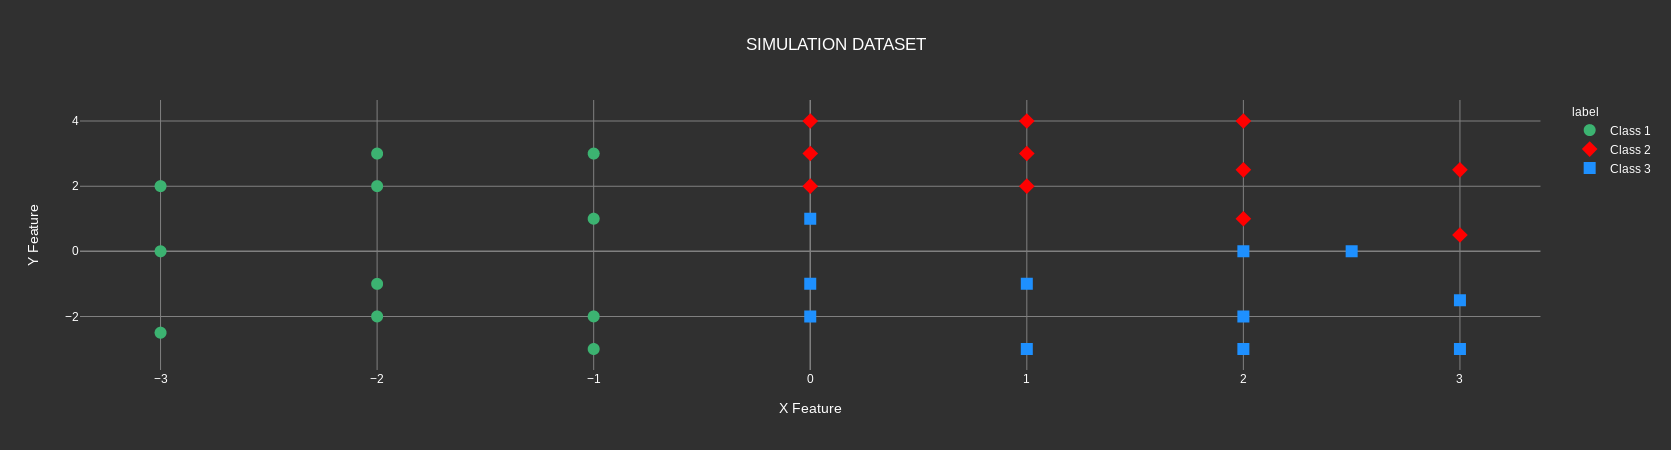
\includegraphics[scale=.2]{./simulation.png}
	
	\subsection{Iris Dataset}
	The Iris Dataset is a common dataset used for beginner problems in machine learning and other areas.  The Iris Dataset comes from MIT, and consists of 150 rows and 4 columns, with a 5th column representing the class of each data point.  The rows of the Iris dataset contains 4 different measurements consisting of "Sepal Length", "Sepal Width", "Petal Length", and "Petal Width", along with the classification of either "Iris Setosa", "Iris Versicolour", or "Iris Virginica".  This dataset is linearly separable between the classes of Iris Setosa and both the other two classes, while it is non linearly separable between Iris Versicolour and Iris Virginica.  This dataset can be visualized in 2D after PCA as follows:\\\\
	\indent\indent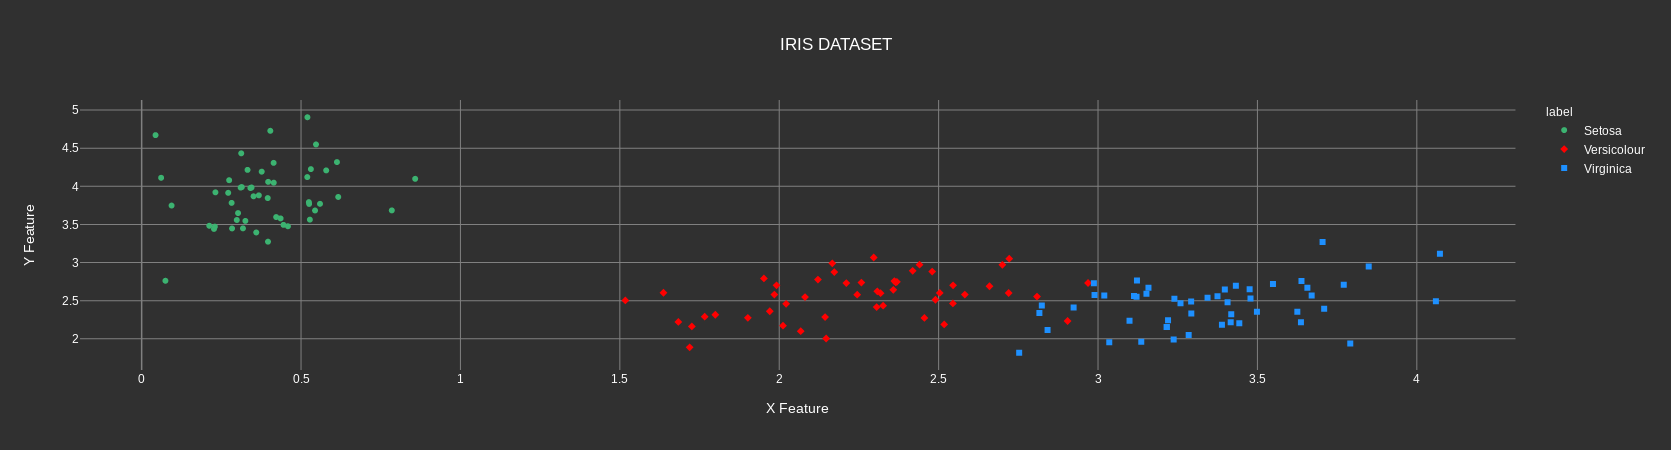
\includegraphics[scale=.2]{./iris.png}
	
	\subsection{Mushroom Dataset}
	A third dataset was used in order to test the algorithm in higher dimensional data.  This dataset originally comes from UCI, but was modified to be used in a binary classification problem of a mushroom being either definitely poisonous, or definitely edible.  This dataset consists of 8124 rows, and 117 columns, with an additional column representing the class of the datapoint.  Each column is a culmination of one-hot-encoded variables, so realistically there are 22 actual features.  An important note is that when classifying a task such as mushroom edibility, the results must be perfectly accurate in order for usability in a real life scenario.  Even one misclassification could contribute to sickness or even fatality, so it is imperative to have accurate results.
	
	\section{Methodology}
	\subsection{Data Cleaning and Transformation}
	The first class created for this project was a class to perform Principle Component Analysis for dimensionality reduction of a given dataset.  This class was used on the Iris Dataset to reduce it to 2 dimensions in order to ease computation and promote visualization.  Each dataset was split into train, and test subsets using the sklearn function "train\_test\_split".  Along with this method, in order to most accurately fit our support vector machine, the X components were standardized about the origin by subtracting the mean of each row and dividing the row by its standard deviation.  Each data point that was fed into the algorithm for testing was also standardized to correspond to the dataset that was originally trained.  Each dataset used was also cleaned up by rows with missing values.
\begin{verbatim}
def split_and_transform(data):
   train, test = train_test_split(data, test_size=0.15)
	
   X_train = np.array(standardize(train.drop(columns=['label'])))
   Y_train = np.array(train['label'])
   X_test = np.array(standardize(test.drop(columns=['label'])))
   Y_test = np.array(test['label'])
	
   return X_train, Y_train, X_test, Y_test
\end{verbatim}
	\subsection{Initialization}
	To create the foundation of the support vector machine model, we created a class/object in python called "SVM".  The SVM is initalized given three hyperparameters corresponding to learning rate, regularization parameter, and max-iterations.
\begin{verbatim}
def __init__(self, learning_rate, regularization_parameter, max_iterations):
   self.learning_rate = learning_rate
   self.C = regularization_parameter
   self.max_iterations = max_iterations
   self.W = None
   self.b = None
\end{verbatim}
	\subsection{Fit Method}
	The next method within the class is called "fit".  The fit method takes in a given dataset along with its classifications, and is where our algorithm is optimized.  The fit function first initializes our weights, w and b, where w is an array of zeros of the length of features, and b is simply set to 0.  We also initialize our sub-gradients of w and b with the same sizes as described before.  Next, our hinge loss is calculated to have an initial value to compare to.  Now, we iterate the amount of times specified by the max-iterations hyperparameter in order to perform subgradient descent.  For each iteration, we update our subgradients with their calculated values, and update our weight parameters.  If we see no significant increase in our hinge-loss, or even a decrease in hinge-loss, we break out of the iterations loop and return our updated parameters.  Otherwise, after all iterations are performed, we update the weights of the class and return.
\begin{verbatim}
def fit(self, X, Y):
   n_features = len(X[0])
   n_samples = len(X)

   self.W = np.array([0.0] * n_features)
   self.b = 0 
   w_grad = np.array([0.0] * n_features)
   b_grad = 0

   hinge_prev = self.hinge_loss(X, Y)

   for i in range(0, self.max_iterations):
      for x_i, y_i in zip(X,Y):
         fx_i = np.dot(self.W, x_i) + self.b
         t = y_i * fx_i

         if (t < 1):
            w_grad += -1 * (y_i * x_i)
            b_grad += -1 * y_i
         else:
            continue

         w_grad = self.W + (self.C * w_grad)
         b_grad = self.C * b_grad

         self.W -= self.learning_rate * w_grad
         self.b -= self.learning_rate * b_grad

         hinge_cur = self.hinge_loss(X, Y)

         if (hinge_cur > hinge_prev and (n_features == 2 or n_features == 3)):
            break

         hinge_prev = hinge_cur

      return
\end{verbatim}
	\subsection{Prediction}
	Our next method is a simple method for classifying any given dataset we've named "predict".  This method returns "1" for a value found above the hyperplane, and returns "-1" for a value found below the hyperplane.
\begin{verbatim}
def predict(self, x):
   return 1 if dot(self.W, transpose(x)) + self.b >= 0 else -1
\end{verbatim}
	\subsection{Accuracy}
	We need a method to test the accuracy of a given support vector machine corresponding to a dataset.  This method calculates the prediction of each data point and compares it to the actual class, and returns a percentage of accuracy.
\begin{verbatim}
def accuracy(self, X, Y):
   successes = 0
   n = len(X)

   for i in range(0, n):
      if (self.predict(X[i]) == Y[i]):
         successes += 1

   return successes / n * 100
\end{verbatim}
	\subsection{Plot}
	The final method within this class is the plot method.  This method utilizes the classes final weights to visualize a 2D representation of the hyperplane, its upper and lower margins, and the dataset that is fed to the class.  The margin can be calculated by the inverse of the norm of the w parameter.
\begin{verbatim}
def plot(self, X, Y):
   data = pd.DataFrame(X)
   dimensions = len(data.columns)
   data['label'] = pd.DataFrame(Y)

   w_norm = np.sqrt(dot(self.W, self.W))
   margin = 1 / w_norm

   min_x = min(data[0])
   max_x = max(data[0])
   min_y = min(data[0])
   max_y = max(data[0])

   x = np.linspace(min_x,max_x,2)
   m = -self.W[0] / self.W[1]
   y = m*x + self.b/self.W[1]
   y_lower = m*x + (self.b - margin)/self.W[1]
   y_upper = m*x + (self.b + margin)/self.W[1]

   plt.scatter(data[0], data[1], c=data['label'].map({-1:'blue',1:'orange'}))
   plt.plot(x, y, 'r')
   plt.plot(x, y_lower, 'g--')
   plt.plot(x, y_upper, 'b--')

   ax = plt.gca()
   ax.set_ylim([min_y / 1.1, max_y * 1.1])

   plt.show()
\end{verbatim}
	\subsection{Dashboard}
	To make visualization and interaction with the algorithm simpler and more involved, a dashboard was created using Python Dash.  This dashboard includes both the simulation dataset, and the Iris dataset, and allows for changes in parameters with real time training and visualization.  This dashboard can be accessed and ran with the github link provided.
	\subsection{Other Notes}
	In order to perform our support vector machine algorithm on a dataset, we need optimal hyperparameters to feed into our fit method.  This can prove difficult to guess without in depth experimentation and experience within the field of data science.  To tackle this issue, we simply specified a list of potential hyperparameters to be tested, and iteratively checked the accuracy of the model after training on our dataset.  This allowed us to obtain the highest accuracy for the model.  The drawback here is that with high dimensional datasets and a slow computer, this could take a significant amount of time, as seen in testing on the mushroom dataset.
	
	\section{Results}
	\subsection{Simulation Results}
	The SVM for the simulation dataset was able to achieve 100\% accuracy on each individual support vector machine with the following weights:\\
	\begin{center}
		\begin{tabular}{||c c c c c c||} 
			\hline
			Classes & Learn Rate & Regularization & Max-Iterations & Weights & Accuracy\\ [0.5ex] 
			\hline\hline
			1, 2 & .01 & 1 & 50 & W: [-1.91,-0.87], b: 0.26 & 100\% \\ 
			\hline
			1, 3 & .01 & 1 & 50 & W: [-2.03,0.25] b: 0.13 & 100\% \\
			\hline
			2, 3 & .001 & .5 & 50 & W: [0.06,1.14] b: -0.04 &100\% \\ [1ex] 
			\hline
		\end{tabular}
	\end{center}
	The final accuracy achieved with multiclass classification of all datapoints was 87.88\%.
	\\
	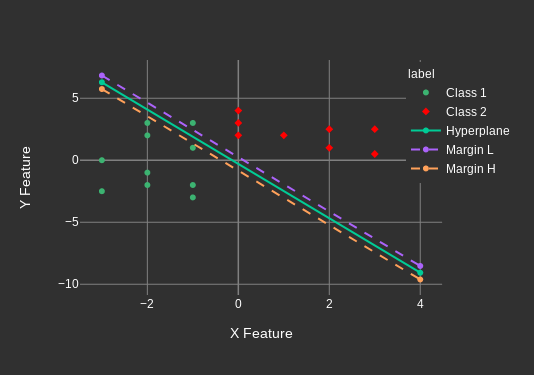
\includegraphics[scale=.3]{./sim1.png}
	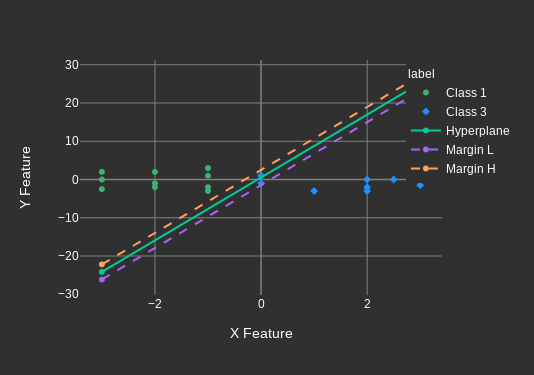
\includegraphics[scale=.3]{./sim2.png}
	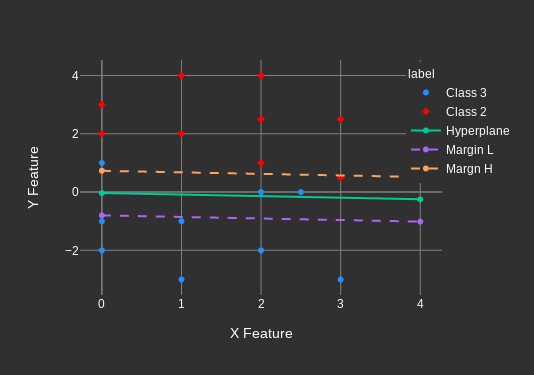
\includegraphics[scale=.3]{./sim3.png}
	\subsection{Iris Results}
	\begin{center}
		\begin{tabular}{||c c c c c c||} 
			\hline
			Classes & Learn Rate & Regularization & Max-Iterations & Weights & Accuracy\\ [0.5ex] 
			\hline\hline
			1, 2 & .01 & 1 & 100 & W: [-2.45,2.36] b: -0.25 & 100\% \\ 
			\hline
			1, 3 & .01 & .25 & 50 & W: [1.31,-0.36] b: -0.15 & 100\% \\
			\hline
			2, 3 & .1 & .25 & 10 & W: [1.72,-1.97] b: -0.06 & 93.33\% \\ [1ex] 
			\hline
		\end{tabular}
	\end{center}
	The final accuracy achived with multiclass classification of all datapoints was 88.00\%.\\
	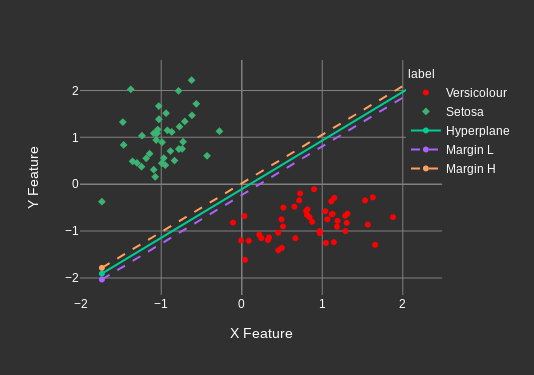
\includegraphics[scale=.3]{./iris1.png}
	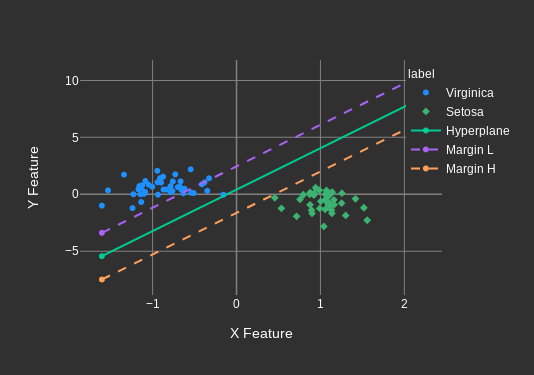
\includegraphics[scale=.3]{./iris2.png}
	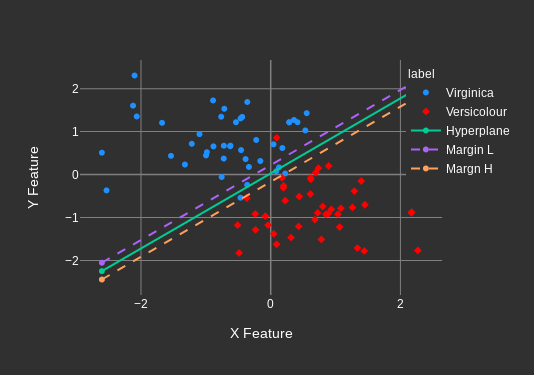
\includegraphics[scale=.3]{./iris3.png}
	
	\subsection{Mushroom Results}
		\begin{center}
		\begin{tabular}{||c c c c c c||} 
			\hline
			Classes & Learn Rate & Regularization & Max-Iterations & Weights & Accuracy\\ [0.5ex] 
			\hline\hline
			1,2 & .001 & .1 & 1000 & (redacted) & 99.753\% \\ [1ex] 
			\hline
		\end{tabular}
	\end{center}
	The weights were removed since it consists of 117 entries for W, but can be found in the jupyter notebook provided in the github link.
	\section{Conclusion}
	Overall the results for binary classification using this support vector machine were substantially accurate.  Very high classification accuracy was achieved in training and testing all of the datasets.  The results for the multiclass classification were a bit under par, and could be improved possibly with a one-vs-all method, or with more personalized tweaks to the methods involved in classification.  The mushroom dataset has good results, but is not recommended for use in a real-life environment as it cannot guarantee perfect results.  The mushroom edibility classification could also be improved with additional accuracy measurements such as keeping track of false-negatives and false-positives, in order to improve it's accuracy for production ready models.
	
\end{document}